\documentclass[a4paper,fleqn]{article}
%
\usepackage{graphicx}
\usepackage{amsmath,amssymb}
%
\graphicspath{{./figures/}}

\title{%
	\bfseries%
	{\large Numerical Techniques Practicum 2}\\[3ex]
	{\Large Solving the advection equation: solutions}
}
%
\author{Daan Degrauwe}
%
\addtolength\textwidth{4cm}
\addtolength\evensidemargin{-2cm}
\addtolength\oddsidemargin{-2cm}
\addtolength\voffset{-2cm}
\addtolength\textheight{4cm}
\setlength\parindent{0pt}
\setlength\parskip{5pt}
\setlength\parsep{5pt}
%
\usepackage{etoolbox}
\makeatletter\preto{\@verbatim}{\topsep=2pt\partopsep=2pt}\makeatother
%
\begin{document}
%
\maketitle
%
\setcounter{section}{1}
%
\section{The upstream scheme}
%
\begin{enumerate}
	\setcounter{enumi}{4}
	\item \textbf{Find 3 ways to make the model unstable}
		%
		\par
		With the original parameter values, the Courant number is $\mu=\frac{c\Delta t}{\Delta x}=0.5$, while the stability condition is $0\leq\mu\leq 1$. To make the model unstable, you can (i) change the direction of the advection, e.g. $c=-0.5$; (ii) increase the time step, e.g. $\Delta t=4.$; (iii) increase the spatial resolution, e.g. $\Delta x=0.25$. The following figures show the results with these parameters.
		%
		\begin{center}
			\hspace*{-50mm}
			\begin{tabular}{ccc}
				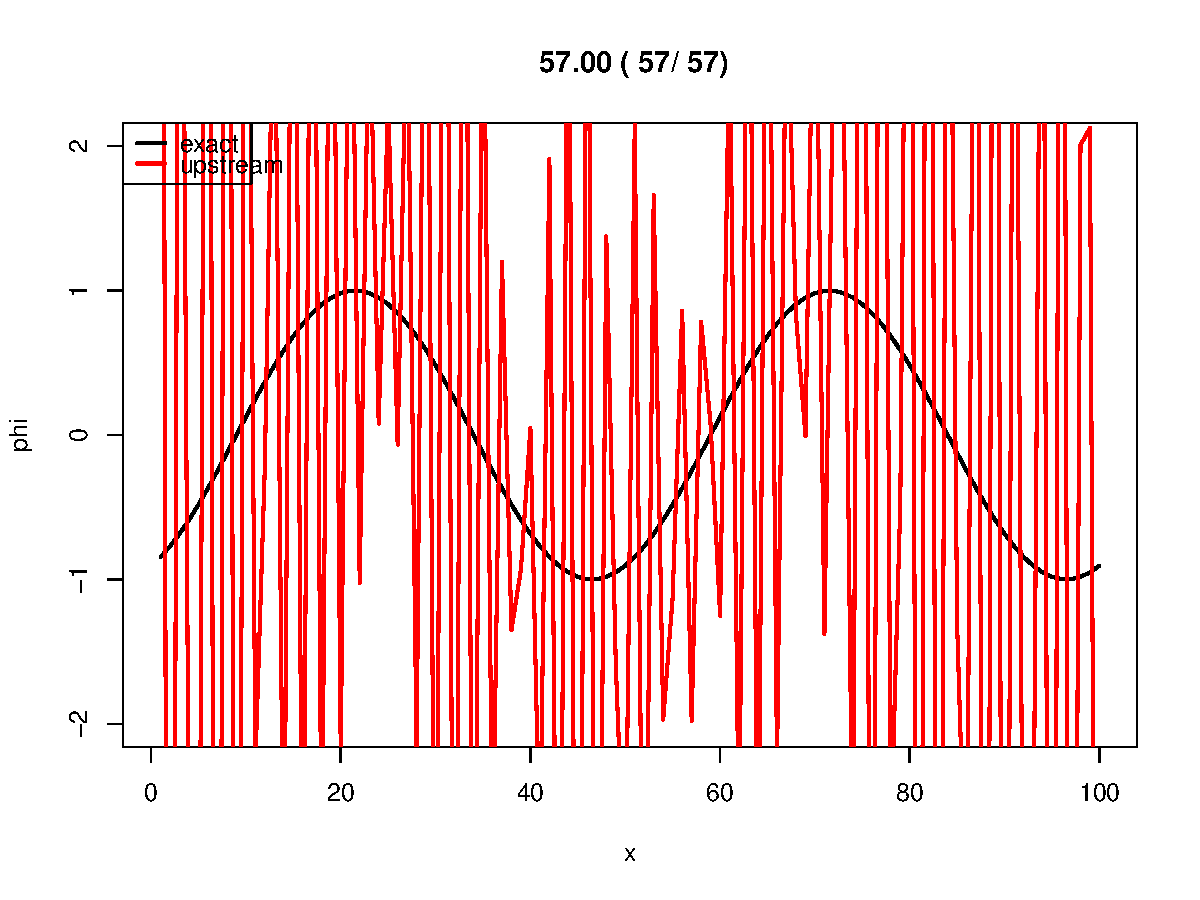
\includegraphics[scale=0.3]{upstream_instab1}	&	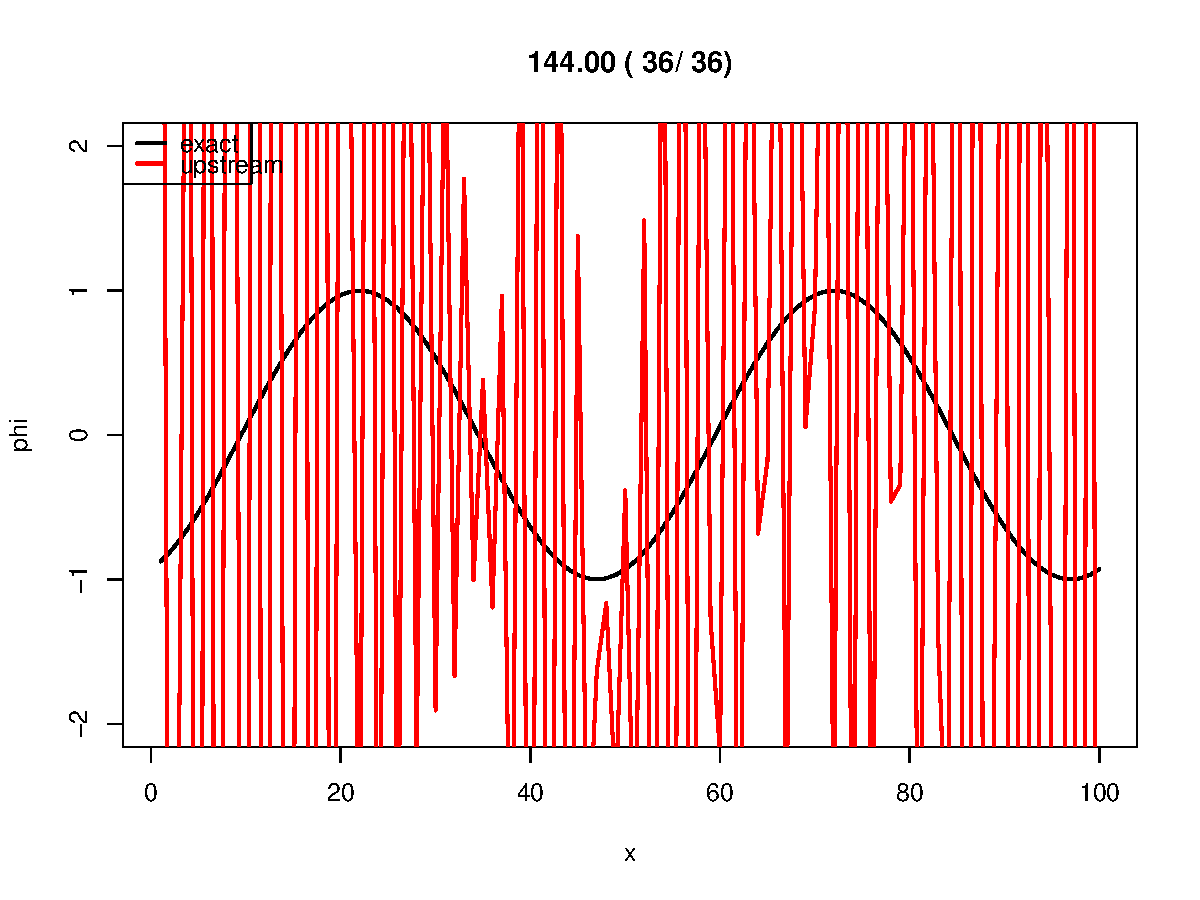
\includegraphics[scale=0.3]{upstream_instab2} & 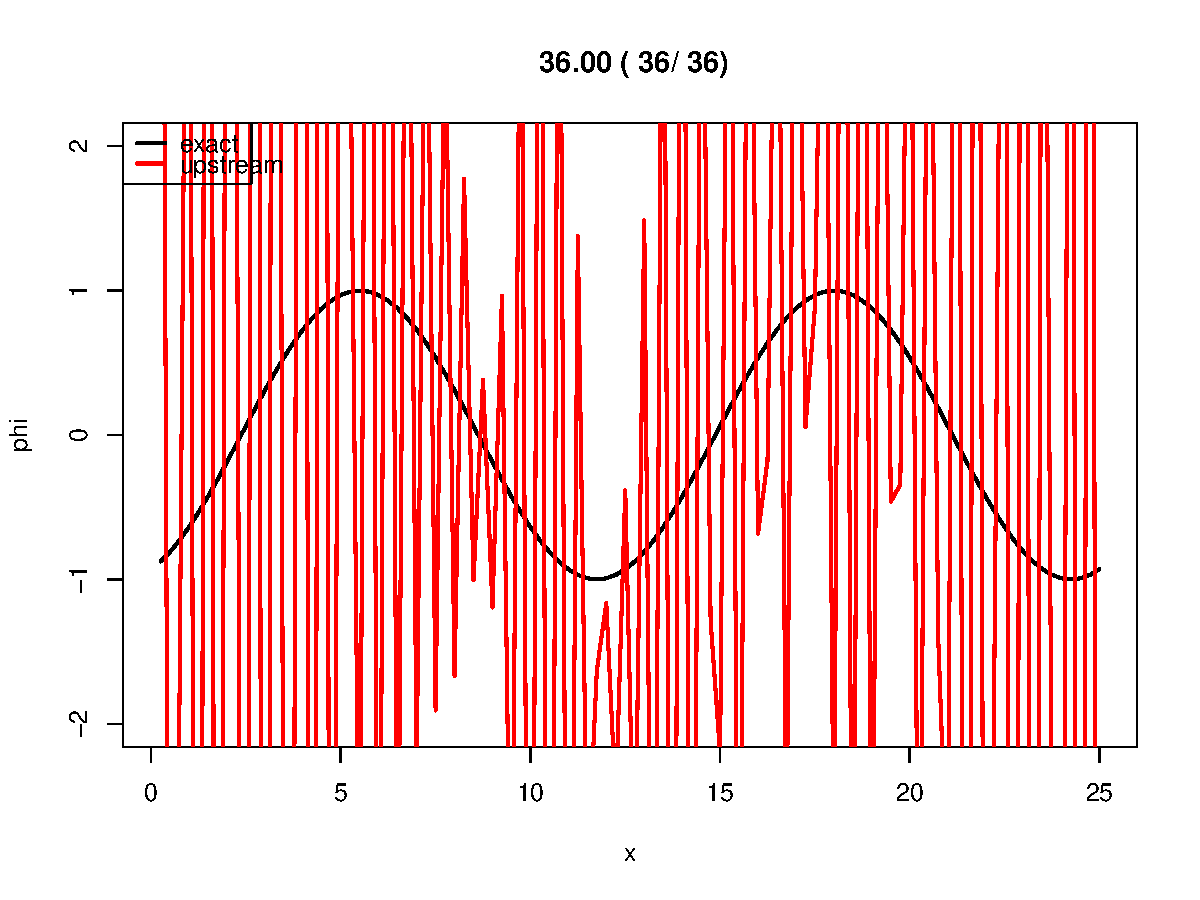
\includegraphics[scale=0.3]{upstream_instab3}\\
				$c=-0.5$	&	$\Delta t=4.0$	&	$\Delta x=0.25$
			\end{tabular}\hspace*{-50mm}
		\end{center}\vspace{2ex}
		%
	\item \textbf{Check the wavelength-dependency of the damping}
		%
		\par
		Shorter waves are damped (or amplified!) more than longer waves. The following figures show the result after 50 timesteps for $KX=2$ and $KX=8$.
		%
		\begin{center}
			\hspace*{-50mm}
			\begin{tabular}{cc}
				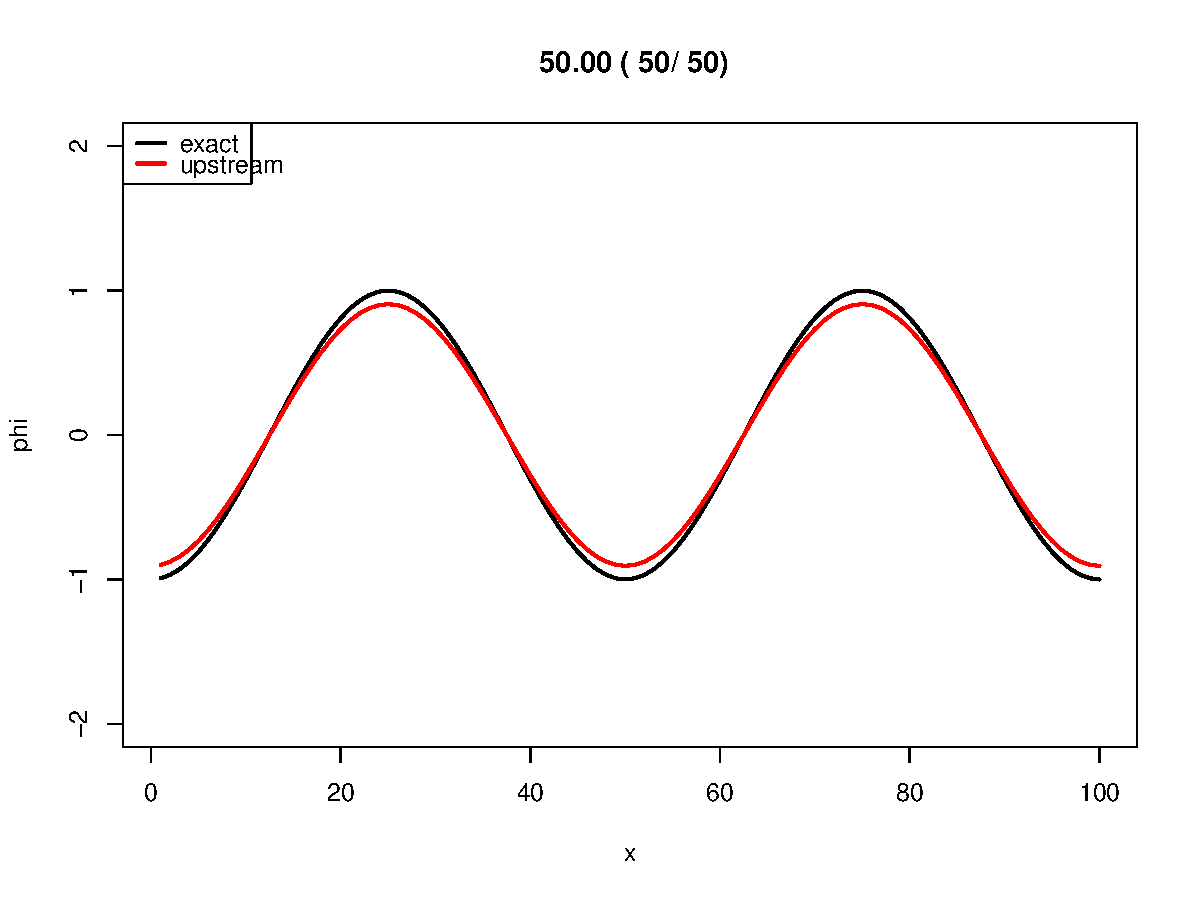
\includegraphics[scale=0.3]{upstream_damp_long}	&	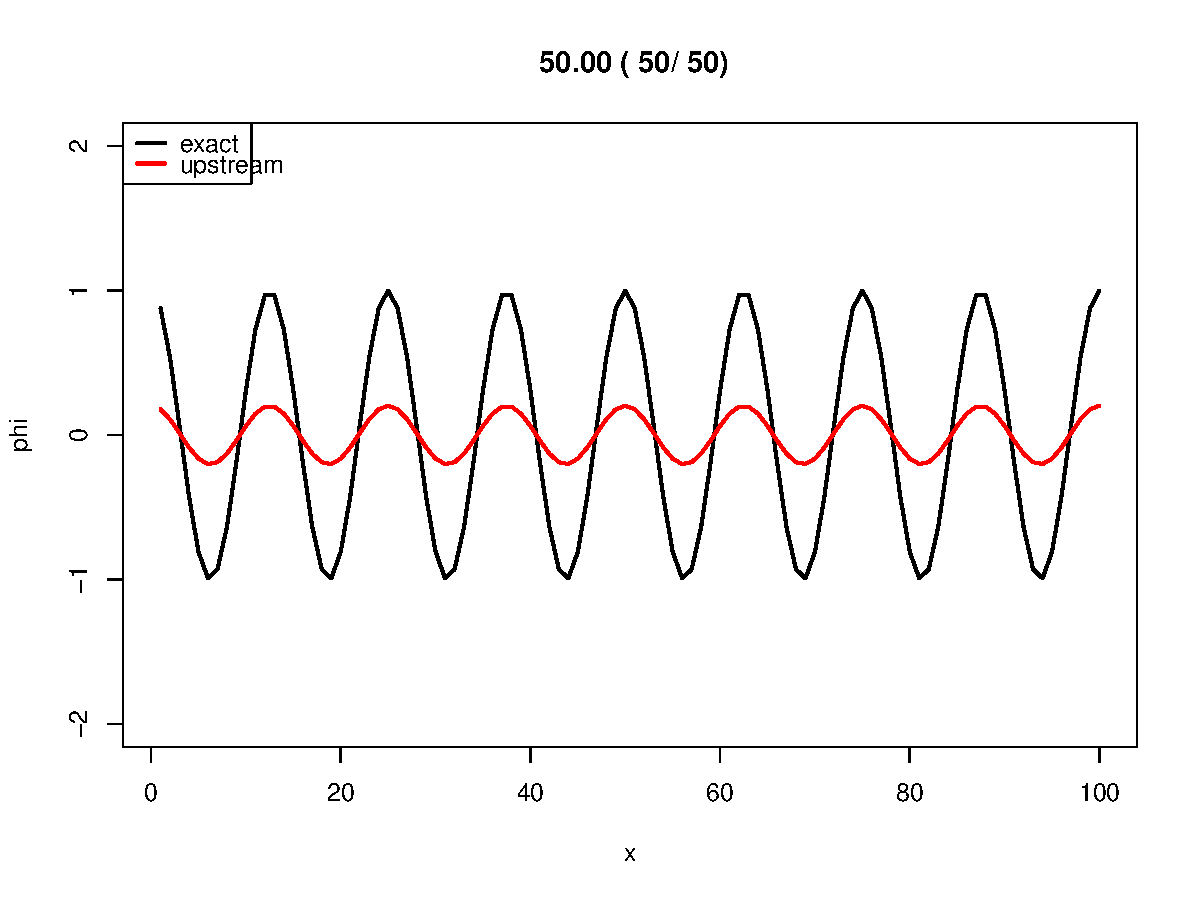
\includegraphics[scale=0.3]{upstream_damp_short}\\
				$KX=2$	&	$KX=8$
			\end{tabular}\hspace*{-50mm}
		\end{center}\vspace{2ex}
		%
	\item \textbf{Why are the shortest waves often the most unstable?}
		%
		\par
		Because for the shortest waves, $k=\pi/\Delta x$, so $\cos k\Delta x$ takes its most extreme value ($-1$).
		%
\end{enumerate}
%
\section{Forward scheme, centered spatial finite differences}
%
\begin{enumerate}
	\setcounter{enumi}{2}
	\item \textbf{Change the spatial discretization into centered finite differences}
		%
		\par
		The modified code can be found on \texttt{helios}, under
		\par
		\texttt{/users/d/ddgrauwe/numtech/2022-2023
\unskip/practica/solutions/adveq/forward\_centered/}\vspace{2ex}
		%
	\setcounter{enumi}{5}
	\item \textbf{ How is it possible that going to a more accurate scheme leads to worse results?}
		%
		\par
		Because in the upstream scheme, errors are compensating: the time scheme is amplifying, but the spatial discretization is damping. Moving to centered spatial finite differences removes the damping (so removes one of the two compensating errors). What remains is the amplification due to the time scheme.
		%
\end{enumerate}
%
\section{Leapfrog time stepping, centered spatial finite differences}
%
\begin{enumerate}
	\item \textbf{Calculate the dispersion relation on paper. What is the stability condition?}
		%
		\par
		The dispersion relation is
		%
		\begin{equation*}
			\omega=\frac{1}{\Delta t}\arcsin\left(\frac{c\Delta t}{\Delta x}\sin k\Delta x\right)
		\end{equation*}
		%
		\par
		The stability condition is
		%
		\begin{equation*}
			\left|\frac{c\Delta t}{\Delta x}\right|\leq1
		\end{equation*}\vspace{2ex}
		%
	\item[2--6.] \textbf{Implement the leapfrog scheme}
		%
		\par
		The modified code can be found on \texttt{helios}, under
		\par
		\texttt{/users/d/ddgrauwe/numtech/2022-2023
\unskip/practica/solutions/adveq/leapfrog\_centered/}\vspace{2ex}
		%
	\setcounter{enumi}{6}
	\item \textbf{Is this scheme accelerating or decelerating?}
		%
		\par
		Decelerating. This can be seen from the dispersion relation ($\omega<ck$) or from running the model.\vspace{2ex}
		%
	\item \textbf{What are the phase speed and group speed for very short waves?}
		%
		\par
		For $k\rightarrow\pi/\Delta x$, the phase speed $\omega/k$ goes to zero, while the group speed $\partial \omega/\partial k$ goes to $-c$.
		%
		\par
		Setting $KX=40$ in \texttt{exact\_solution.F90} will show you that the phase speed for this wavenumber is close to zero.\vspace{2ex}
		%
	\item \textbf{Visualizing the group speed}
		%
		\par
		In \texttt{exact\_solution.F90}, put the line
		%
		\begin{verbatim}
		   PSI(IX) = COS(2*PI*48*(IX*DX-C*T)/LX)+COS(2*PI*49*(IX*DX-C*T)/LX)
		\end{verbatim}
		%
		The result looks a bit random (because these waves are on the limit of what can be represented on this resolution), but you should be able to see the energy moving in the wrong direction.
		%
\end{enumerate}
%
%\end{document}
\section{Heun and Matsuno with centered spatial differences}
%

\begin{enumerate}
	\item \textbf{The Heun scheme}
		%
		\par
		The code for this scheme can be found on \texttt{helios}, under
		\par
		\texttt{/users/d/ddgrauwe/numtech/2022-2023
\unskip/practica/solutions/adveq/heun\_centered/}
		%
		\par
		Following figures show the results with the Heun scheme for $\mu=0.8$. For long waves, the amplification is very weak (even after 500 timesteps). Shorter waves are more unstable (crash after 58 timesteps).
		%
		\begin{center}
			\hspace*{-50mm}
			\begin{tabular}{cc}
				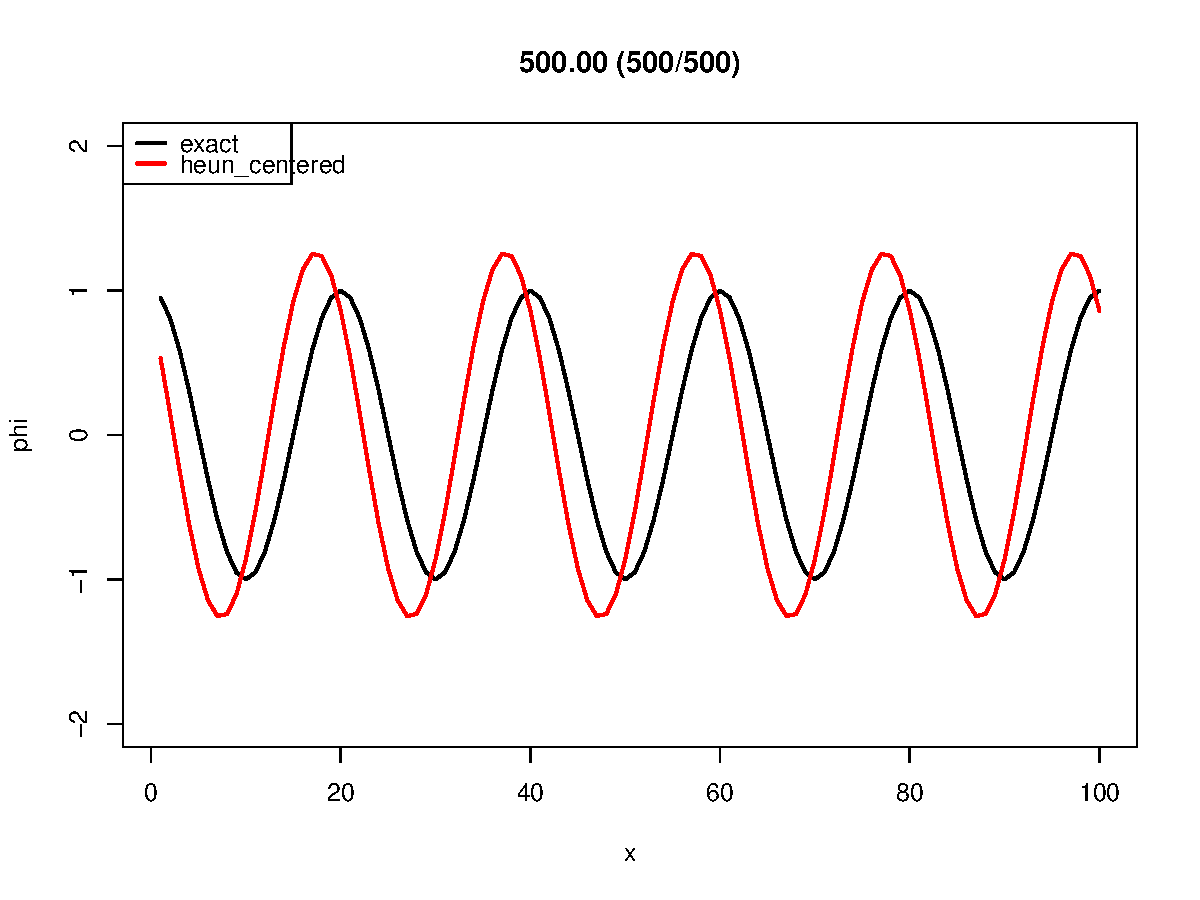
\includegraphics[scale=0.3]{heun_long}	&	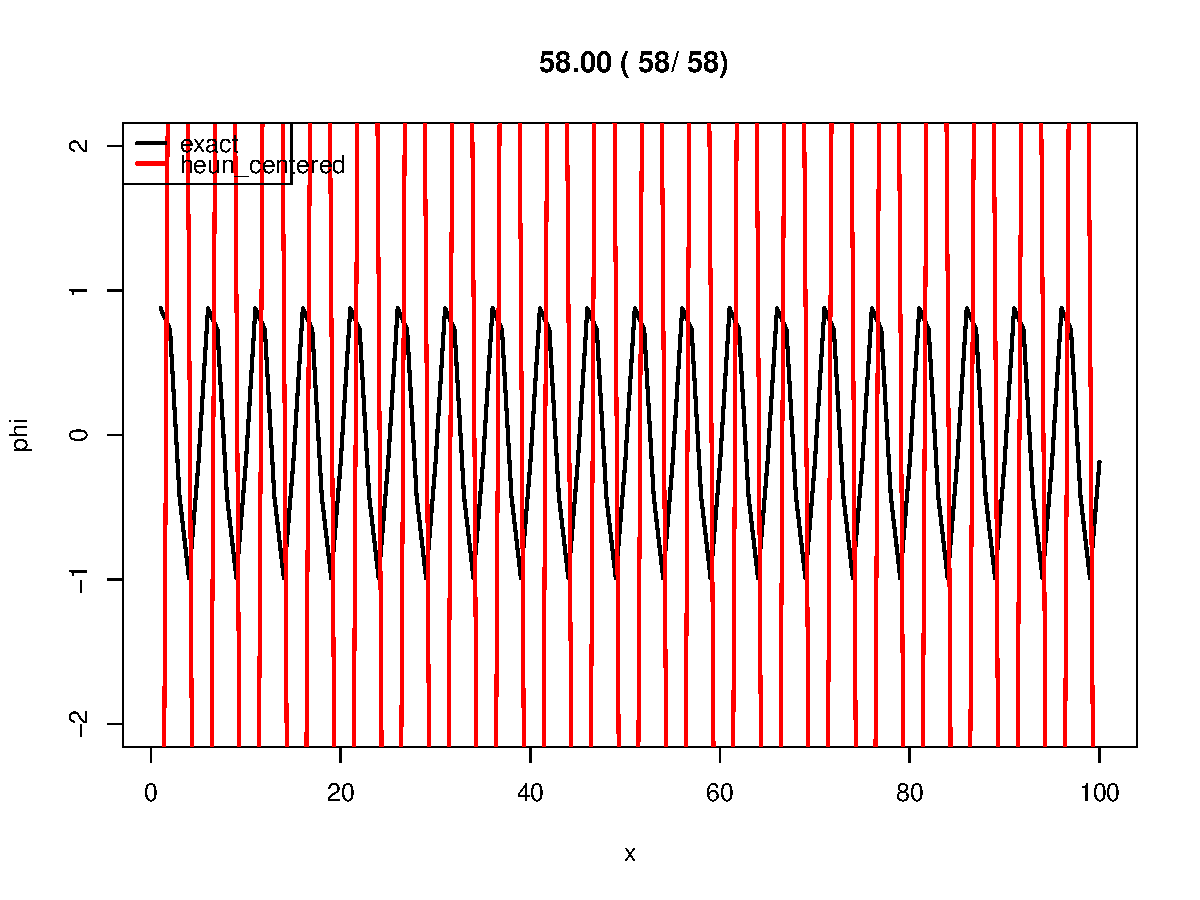
\includegraphics[scale=0.3]{heun_short}\\
				$KX=5$	&	$KX=20$
			\end{tabular}\hspace*{-50mm}
		\end{center}\vspace{2ex}
		%
	\item \textbf{The Matsuno scheme}
		\par
		The code for this scheme can be found on \texttt{helios}, under
		\par
		\texttt{/users/d/ddgrauwe/numtech/2022-2023
\unskip/practica/solutions/adveq/matsuno\_centered/}
		%
		\par
		Following figures show the results with the Matsuno scheme for $\mu=0.8$. Long and short waves have little damping, while intermediate waves undergo stronger damping.
		%
		\par
		\begin{center}
			\hspace*{-50mm}
			\begin{tabular}{ccc}
				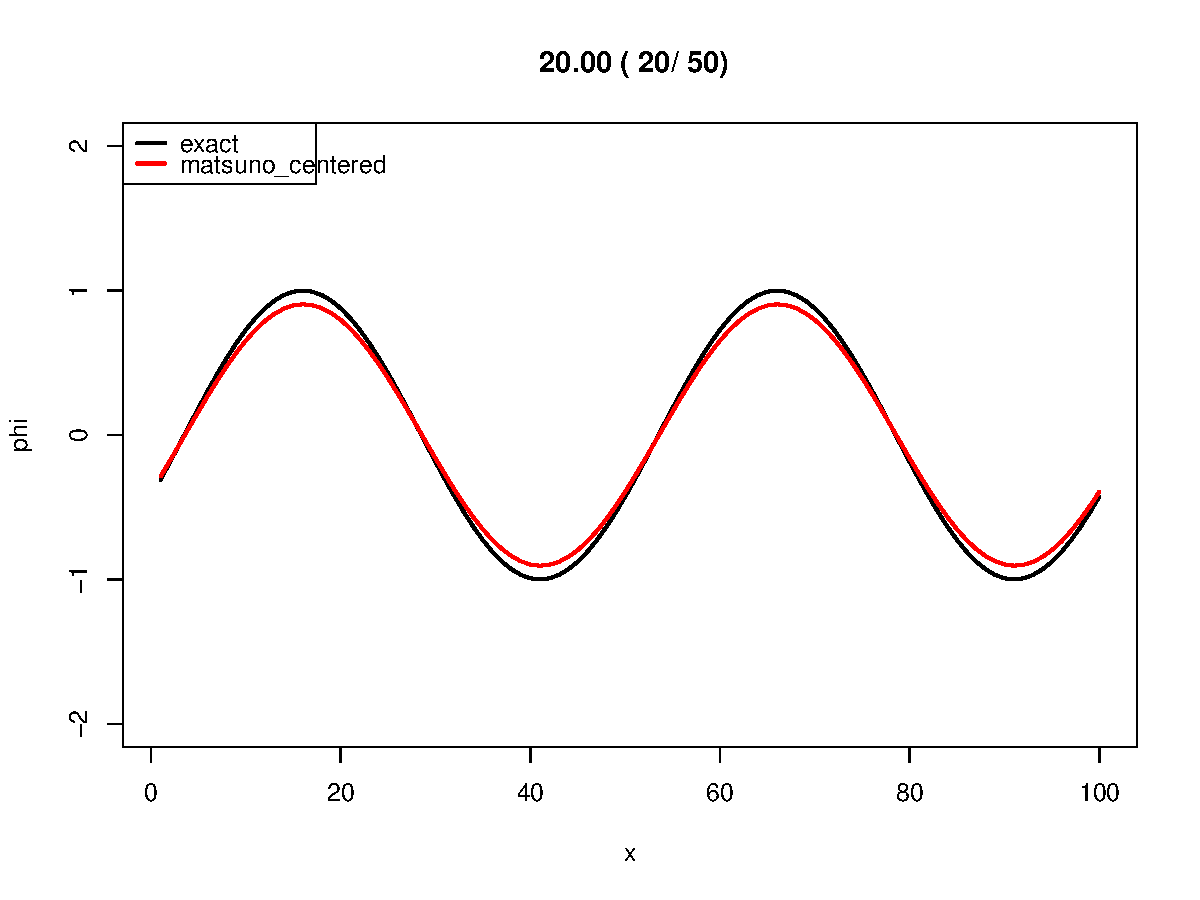
\includegraphics[scale=0.3]{matsuno_long}	& 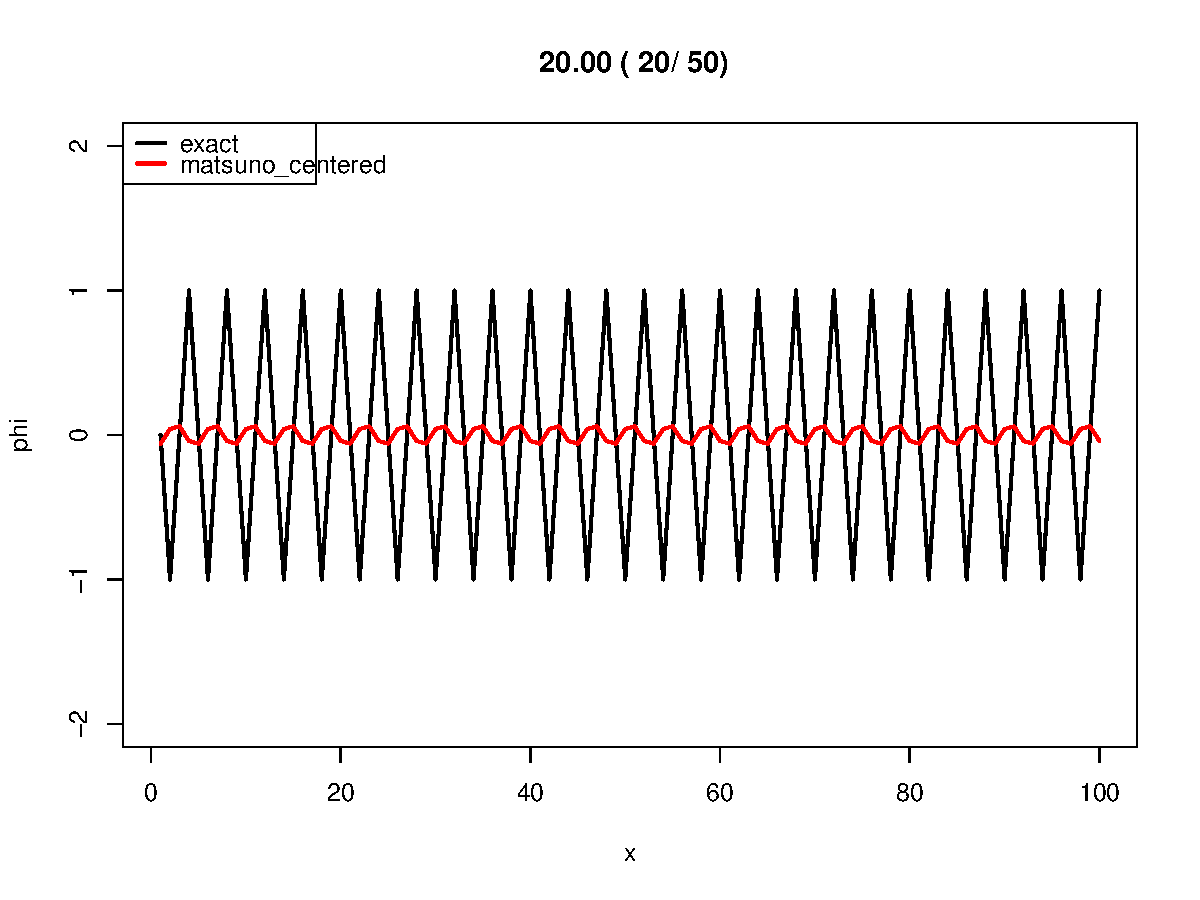
\includegraphics[scale=0.3]{matsuno_medium}	&	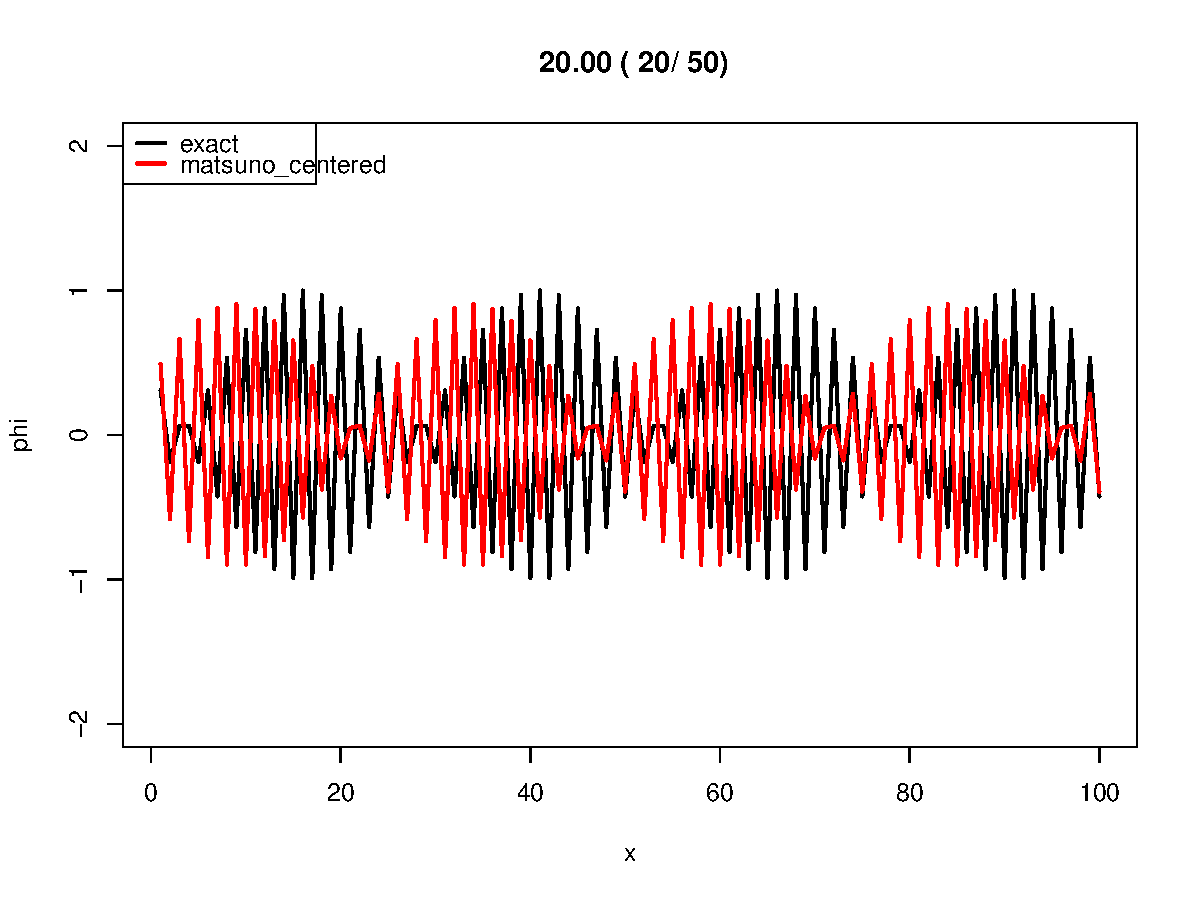
\includegraphics[scale=0.3]{matsuno_short}\\
				$KX=2$	&	$KX=25$	&	$KX=48$
			\end{tabular}\hspace*{-50mm}
		\end{center}
		%
\end{enumerate}
%
\section{Spectral model}
%
\begin{enumerate}
	\item \textbf{Changing upstream to trapezium scheme}
		%
		\par
		The challenge is that the trapezium scheme is an implicit scheme: values at the next timestep ($\phi^{n+1}$) appear multiple times in the equation. For instance, in order to calculate $\phi^{n+1}_j$, one needs $\phi^{n+1}_{j-1}$. But to determine $\phi^{n+1}_{j-1}$, one needs \ldots $\phi^{n+1}_j$. So all gridpoints are \emph{coupled}.
		%
		\par
		In order to solve such a system, the scheme is written as:
		%
		\begin{equation*}
			-\tfrac{\mu}{4}\phi_{j-1}^{n+1}+\phi_j^{n+1}+\tfrac{\mu}{4}\phi_{j-1}^{n+1} = \tfrac{\mu}{4}\phi_{j-1}^{n+1}+\phi_j^{n+1}-\tfrac{\mu}{4}\phi_{j-1}^{n+1}
		\end{equation*}
		%
		Putting such equations together for all gridpoints (i.e. $j=1,\ldots,n$) results in the following tridiagonal linear system of equations:
		%
		\begin{equation*}
			\left(\begin{array}{ccccc}
				1 & & \cdots & & -\tfrac{\mu}{4}	\\
				&\ddots&&&	\\
					& -\tfrac{\mu}{4}	&	1	&	\tfrac{\mu}{4}	&	\\
				&&&\ddots&\\
				\tfrac{\mu}{4}	&&	\cdots	&&	1
			\end{array}\right)
			\left(\begin{array}{c}
				\phi_1	\\	\vdots \\	\phi_{j-1}	\\	\phi_{j}	\\	\phi_{j+1}	\\	\vdots \\ \phi_n
			\end{array}\right)
			=
			\left(\begin{array}{ccccc}
				1 & & \cdots & & \tfrac{\mu}{4}	\\
				&\ddots&&&	\\
					& \tfrac{\mu}{4}	&	1	&	-\tfrac{\mu}{4}	&	\\
				&&&\ddots&\\
				-\tfrac{\mu}{4}	&&	\cdots	&&	1
			\end{array}\right)
			\left(\begin{array}{c}
				\phi_1	\\	\vdots \\	\phi_{j-1}	\\	\phi_{j}	\\	\phi_{j+1}	\\	\vdots \\ \phi_n
			\end{array}\right)
		\end{equation*}
		%
		If you think writing out this system is hard, try solving it ;-) Although efficient techniques exist for solving tridiagonal systems, it remains a daunting job, especially for 2D or 3D problems.\vspace{2ex}
		%
	\setcounter{enumi}{3}
	\item \textbf{How is it possible that changing to a more accurate space discretization gives worse results?}
		%
		\par
		Because of the compensating errors in the upstream scheme. Taking one error away (damping effect of the spatial discretization) then gives worse results.\vspace{2ex}
		%
	\item \textbf{Implement trapezium timestepping}
		%
		\par
		The code for this scheme can be found on \texttt{helios}, under
		\par
		\texttt{/users/d/ddgrauwe/numtech/2022-2023
\unskip/practica/solutions/adveq/trapezium\_spectral}
		%
		\par
		This scheme is unconditionally stable. Since the $\arctan$ function gives a real result for any (real) argument, the frequency $\omega$ will be a real number for any wavenumber $k$. This means that the imaginary component of $\omega$ is zero, meaning there is no amplitude error (damping or amplification).
		%
\end{enumerate}
%
\end{document}
%
